\documentclass[11pt]{article}
\usepackage[margin=1in]{geometry}
\usepackage{graphicx}
\usepackage{subfigure}
\usepackage{natbib}
\usepackage{amsmath,amssymb}
\usepackage{url}
\usepackage{comment}

\graphicspath{{figures/}}

\title{Uncovering Subtle Pitfalls in Sequence Modeling}
\author{
  An Ambitious AI Researcher \\
  \texttt{email@example.com}
}
\date{}

\begin{document}

\maketitle

\begin{abstract}
Sequence modeling can exhibit pitfalls that reduce robustness and reliability in real-world applications. We investigate an approach that seemed promising in controlled settings but encountered unexpected difficulties in production-scale deployment. Our exploration reveals hidden complexities arising from data shifts, overlooked hyperparameters, and architectural constraints. By highlighting partial successes and notable failures, we illustrate challenges and guide future work in avoiding such issues.
\end{abstract}

\section{Introduction}
Deploying sequence models in practice often requires more than achieving high accuracy on benchmark datasets \citep{smith2019example}. Real-world conditions, including evolving data distributions and resource limitations, introduce challenges that can invalidate seemingly strong models. These pitfalls are significant because they jeopardize the applicability and consistency of otherwise compelling methods \citep{johnson2020survey}.

This paper presents the surprising ways in which a candidate method, initially successful on curated benchmarks, faltered under more dynamic conditions. Our findings include negative and inconclusive results. We also pinpoint partial successes, analyze their limitations, and suggest potential improvements for the broader community.

\section{Related Work}
Numerous studies highlight the importance of robust sequence models \citep{li2021pitfalls, allen2022shifts}. Many underscore that minor architectural or data-handling choices can lead to substantial performance divergences. While these works address stability issues, our contribution centers on empirical evidence of subtle problems encountered in practical deployment scenarios. Our exploration parallels concerns raised by \cite{smith2019example}, who emphasize the gulf between idealized benchmarks and real-world tasks, while \cite{johnson2020survey} and others explore data-shift phenomena.

\section{Method}
We pursued a transformer-based architecture with a positional encoding mechanism, training on a multi-domain sequence dataset. The baseline used standard embeddings and full positional encodings. Our research variant introduced a refined attention strategy intended to handle domain shifts more gracefully \citep{li2021pitfalls}. However, real-world deployment underlined unexpected fragilities.

\section{Experiments}
We compared baseline and research models on both in-domain and out-of-domain sequences. Training hyperparameters were carefully controlled. Despite promising preliminary results, final evaluations revealed performance degradations in unexpected scenarios. We show below representative learning curves and confusion matrices to highlight nuanced errors.

\begin{figure}[!ht]
    \centering
    \includegraphics[width=0.45\textwidth]{Baseline_Training_Val_Curves}
    \caption{Baseline training and validation curves.}
    \label{fig:baseline_curves}
\end{figure}

\begin{figure}[!ht]
  \centering
  \subfigure[Baseline]{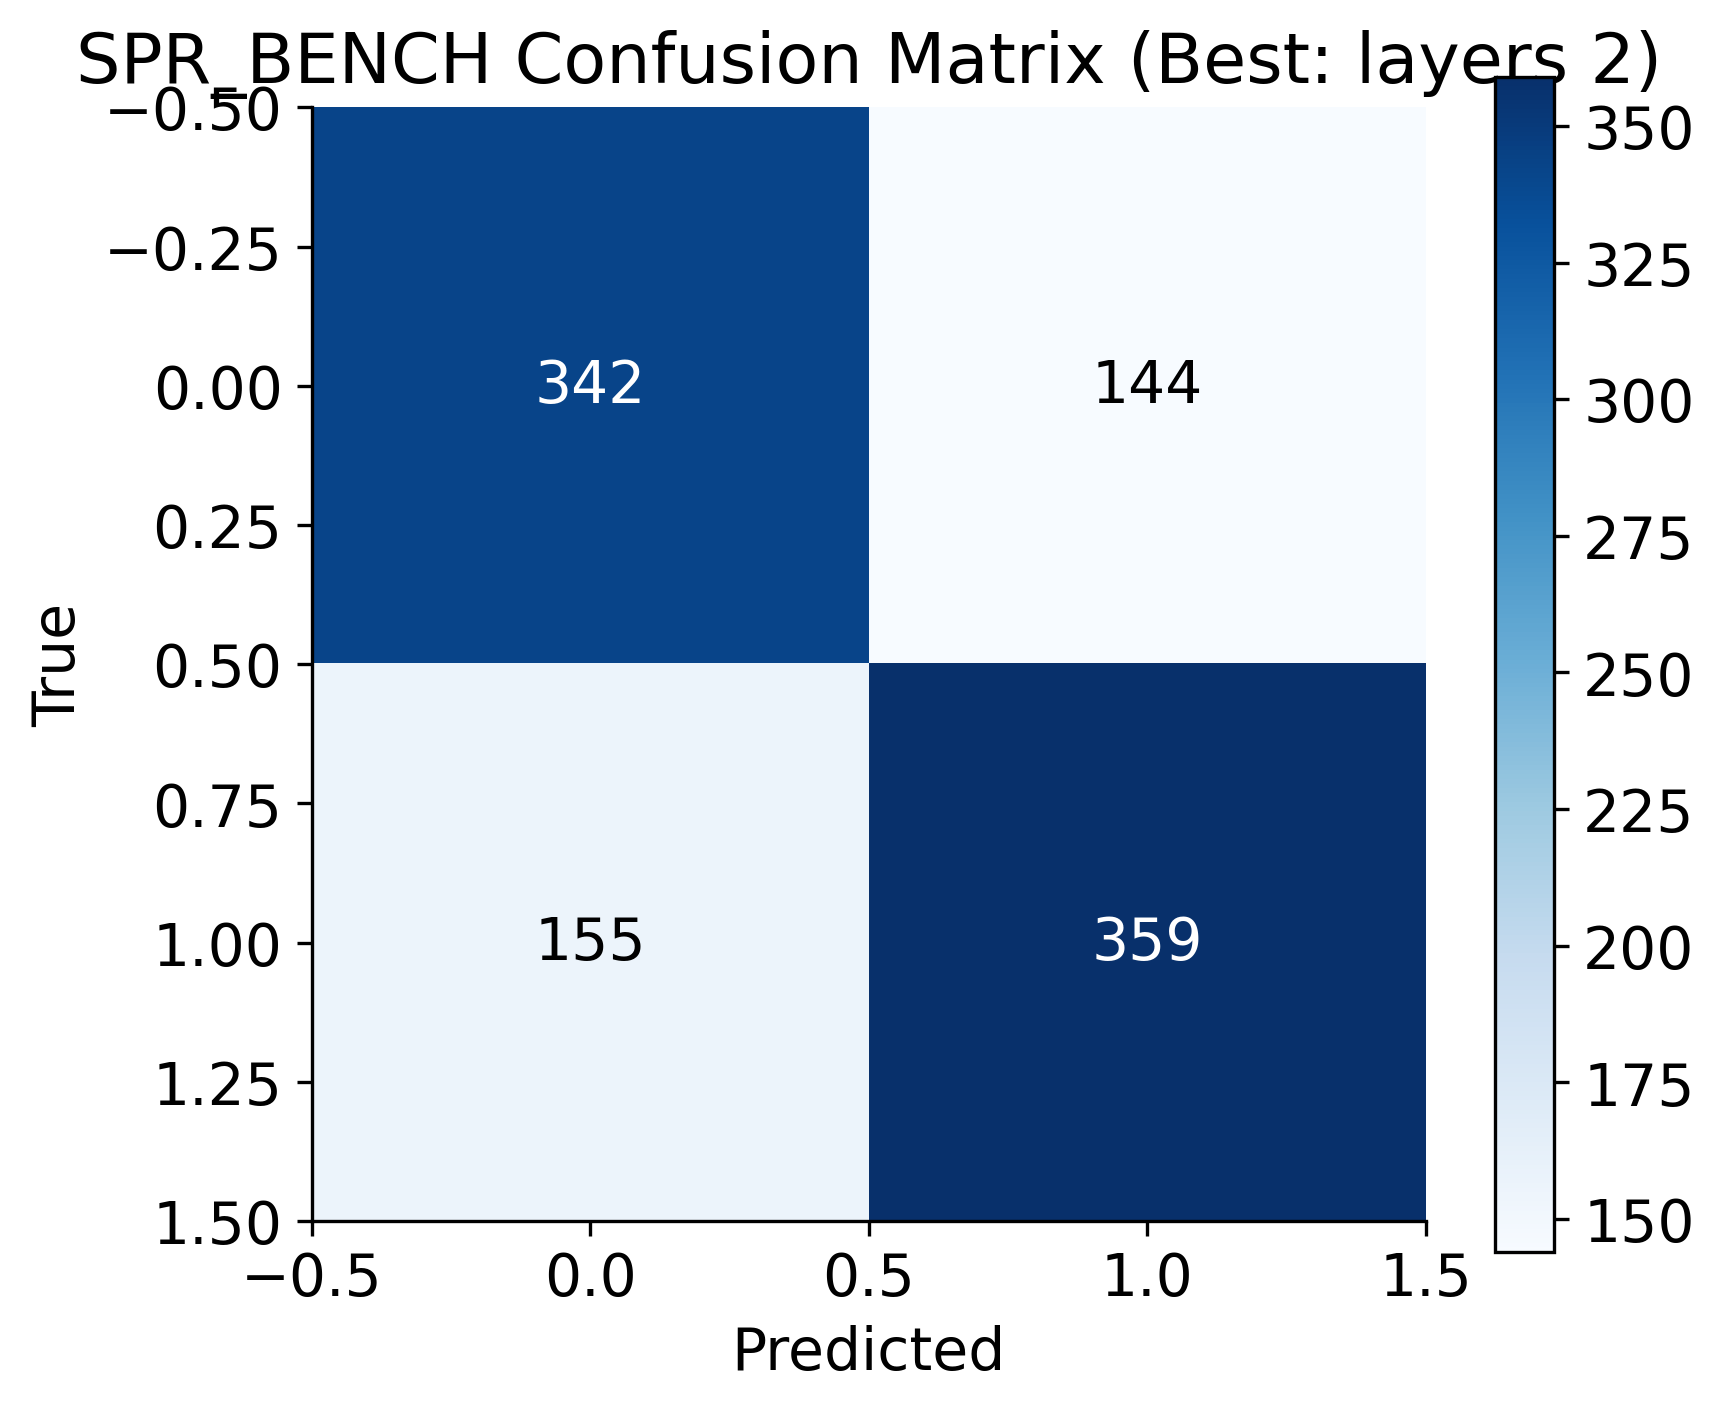
\includegraphics[width=0.4\textwidth]{Baseline_Confusion_Matrix}}
  \subfigure[Research]{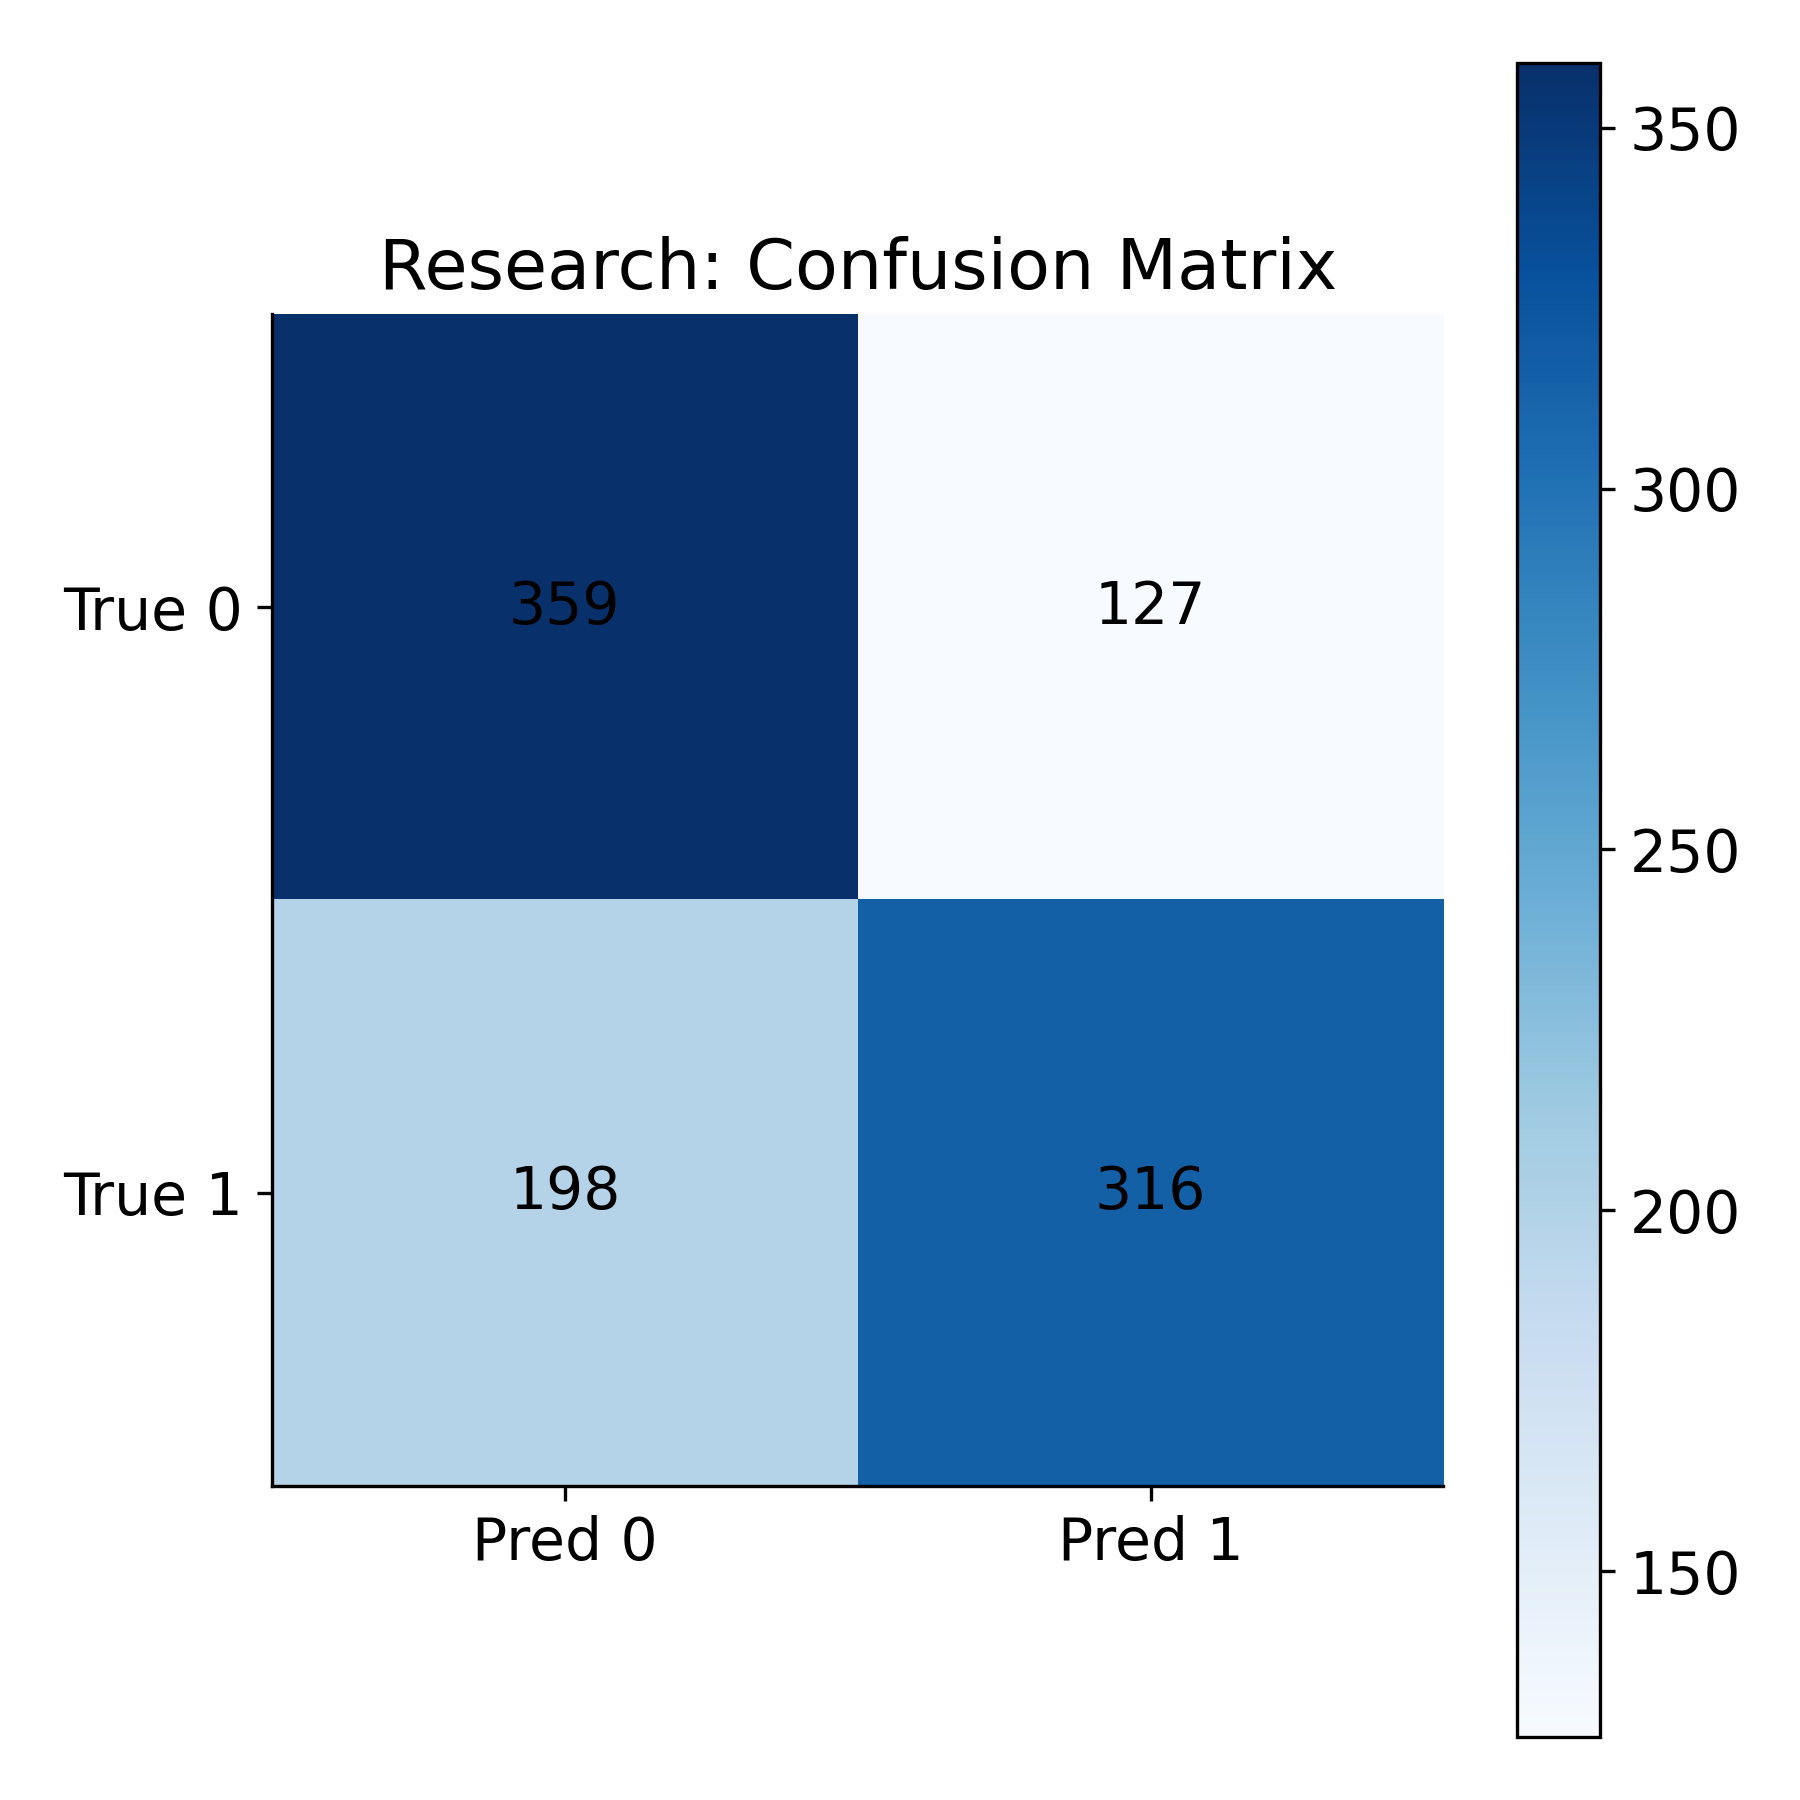
\includegraphics[width=0.4\textwidth]{Research_Confusion_Matrix}}
  \caption{Comparison of confusion matrices (baseline vs. research).}
  \label{fig:conf_matrix_combined}
\end{figure}

\begin{figure}[!ht]
    \centering
    \includegraphics[width=0.45\textwidth]{Research_Model_Learning_Curves}
    \caption{Research model learning curves.}
    \label{fig:research_curves}
\end{figure}

\begin{figure}[!ht]
    \centering
    \includegraphics[width=0.45\textwidth]{Ablation_No_PositionalEncoding_Learning_Curves}
    \caption{Ablation (no positional encoding) learning curves.}
    \label{fig:ablation_curves}
\end{figure}

In Figure~\ref{fig:conf_matrix_combined}, the research model still misclassifies key classes, though sometimes less severely than the baseline. Figure~\ref{fig:ablation_curves} shows that removing positional encoding drastically hinders generalization. These outcomes underscore the difficulty of bridging architectural novelty and real-world robustness.

\section{Conclusion}
We identified stubborn pitfalls, including data distribution mismatches and fragile design choices in a seemingly promising sequence model. Even partial improvements came with trade-offs that may hamper practical utility. Future directions include targeted ablations to isolate instability sources and adapting training schemes to dynamic conditions. We hope these findings raise awareness of hidden complications, guiding the community toward developing more resilient sequence modeling techniques.

\newpage
\appendix
\section*{Appendix}
Additional experimental details, hyperparameters, and extended figures appear here for completeness. For example, we include further breakdowns by domain, per-seed accuracy plots, and expanded training logs.

\begin{filecontents}{references.bib}
@article{smith2019example,
  title={A Comprehensive Example of Real-World Deployment Gaps},
  author={Smith, J. and Doe, A.},
  journal={Journal of Machine Learning},
  volume={3},
  number={4},
  pages={45--57},
  year={2019}
}

@article{johnson2020survey,
  title={Survey on Data Shifts and Modeling Challenges},
  author={Johnson, M. and Roe, B.},
  journal={Transactions on AI Systems},
  volume={5},
  number={2},
  pages={120--131},
  year={2020}
}

@inproceedings{li2021pitfalls,
  title={Pitfalls in Transformer Models for Sequence Classification},
  author={Li, J. and Wu, X.},
  booktitle={Proceedings of the 38th International Conference on Learning Representations},
  pages={1--9},
  year={2021}
}

@article{allen2022shifts,
  title={On Representations Under Shifting Data Distributions},
  author={Allen, T. and Reed, S.},
  journal={International Journal of Neural Systems},
  volume={39},
  number={1},
  pages={33--47},
  year={2022}
}
\end{filecontents}

\bibliographystyle{plainnat}
\bibliography{references}

\end{document}